%analysis body
%Created MB 04-12

\section{Analysis}\label{analysis}
\subsection{Second Sound Analysis}\label{secondsoundanalysis}

We determine the relationship between the temperature of He II and the propagation speed of second sound by analyzing the second sound data shown in Fig. \ref{fig:secondsoundraw}. Using linear regression analysis, we determine the slope of each temperature data set.  For each of the fifteen data sets, the $r^{2}$-value is greater than $0.99$.  The values for the slope of these fits, in m/s, correspond to the propagation speed of second sound in the respective temperature.  These speeds are plotted against temperature in order to show the relationship between the two in He II (Fig. \ref{fig:secondsound}).  This data is compared to results made by Peshkov \cite{peshkov}.
\begin{figure}[htbp]
\begin{center}
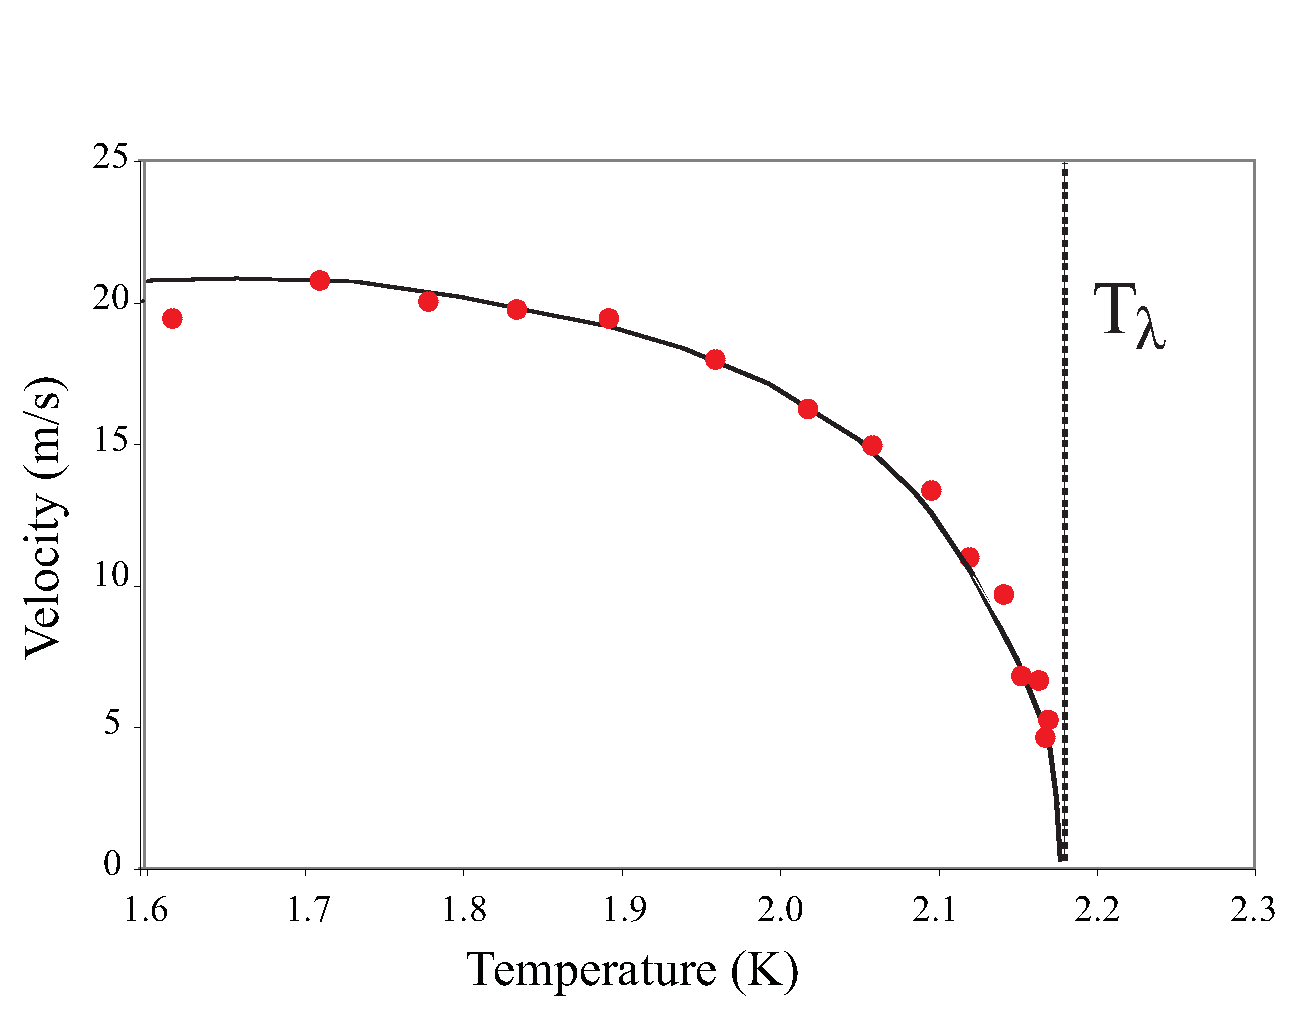
\includegraphics[height=70mm]{./figures/secondsound.eps}
\caption{\small{A plot of the second sound speed verses temperature in He II.  This data is compared to Peshkov's results\cite{peshkov}. Second sound velocity goes to zero at the transition from He II to He I, enabling a rough estimate of $T_{\lambda}$.}}
\label{fig:secondsound}
\end{center}
\end{figure}

The statistical error of the speeds is due to statistical measurement error, resulting in a relative error of $2.1\%$. To eliminate systematic error in second sound calculations, we calculate the slope of several measurements of time delay \emph{vs.} measured displacement of the bolometer. This method avoids systematic offsets to either the time delay or the displacement and instead emphasizes the relative differences between data points. As a result, the error in second sound speed is purely statistical (see Appendix \ref{errorinsecondsoundcalculation} for further error analysis).

\subsection{Heat Capacity Analysis}\label{heatcapacityanalysis}
\subsubsection{Temperature Calibration}\label{temperaturecalibration}

In order to measure heat capacity, we must be able to measure the temperature of the cell.  Because the germanium resistor is thermally coupled to the cell, we can use it as a thermometer for the cell.  Therefore, the potential difference across the resistor must be converted to temperature.  Following the procedure described in Section \ref{thermometercalibration}, data relating the potential difference across the resistor to the vapor pressure of the bath is produced.  The pressure is measured by two separate gauges which report pressures over different ranges. These pressures are calibrated in order to be in agreement with a previously established absolute pressure calibration.  The corresponding temperature of the thermometer is determined through the vapor pressure of the bath. The resulting temperature \emph{vs.} potential data is fit to a curve given by Eqn. \ref{eq:fiteqn} in order to determine an analytic expression for temperature as a function of electric potential. This data is shown with the fit in Fig. \ref{fig:polyfit}.  
\begin{figure}[htbp]
\begin{center}
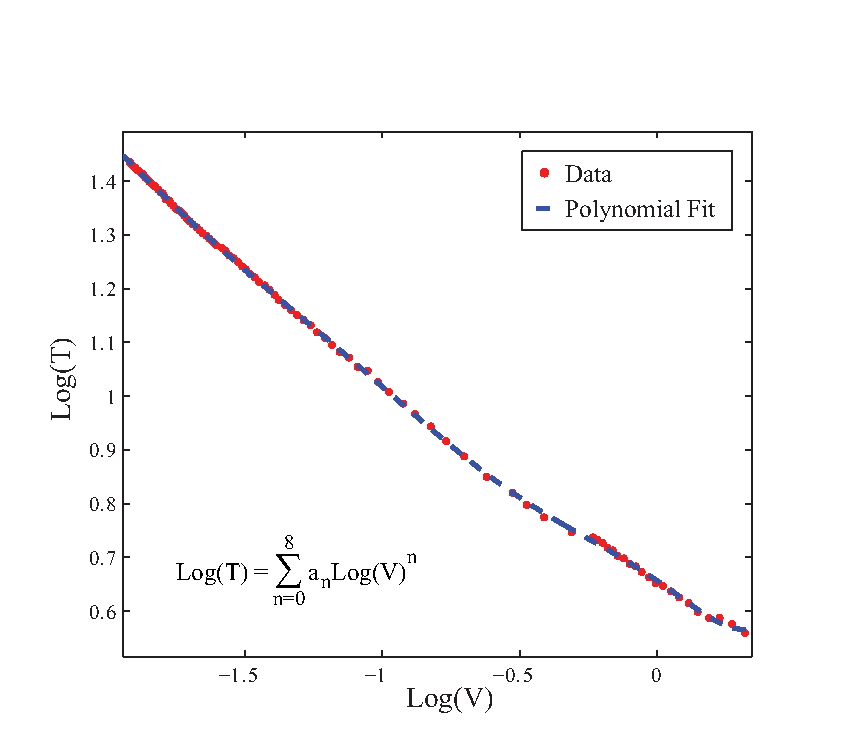
\includegraphics[height=70mm]{./figures/polyfit.eps}
\caption{\small{Log-log relationship between the potential difference across the germanium resistor and the temperature of the cell.  The $8^{th}$-degree polynomial nonlinear regression analysis fit is based on Eqn. \ref{eq:fiteqn}. The resultant $r^{2}$-value is $0.999$.}}
\label{fig:polyfit}
\end{center}
\end{figure}

The fit was computed using a $8^{th}$-degree polynomial regression (see Appendix \ref{nonlinearregressionanalysis}) of the log-log data and found to be 
\begin{eqnarray}\label{eq:polyfit}
\ln(T) &=& 0.6568 - 0.3503\ln(V) - 0.1635\ln(V)^{2} + 0.2846\ln(V)^{3} \\
& & + 1.813\ln(V)^{4} + 2.521\ln(V)^{5} + 1.593\ln(V)^{6} + 0.4845\ln(V)^{7} + 0.0578\ln(V)^{8} \nonumber
\end{eqnarray}

where $T$ is the temperature of the cell and $V$ is the potential difference across the germanium resistor.  Relative uncertainties in the fitting parameters of this polynomial contribute to the relative error in calculated temperatures.   

\subsubsection{Calculating the Heat Capacity of Helium}\label{calculatingtheheatcapacityofthecell}

In order to calculate heat capacity from the data shown in Fig. \ref{fig:rawdata}, the potential difference across the germanium resistor must be converted to temperature using Eqn. \ref{eq:polyfit} determined in Section \ref{temperaturecalibration}. A portion of the sample data after being converted from potential to temperature is shown in Fig. \ref{fig:heatingdata}.  
\begin{figure}[htbp]
\begin{center}
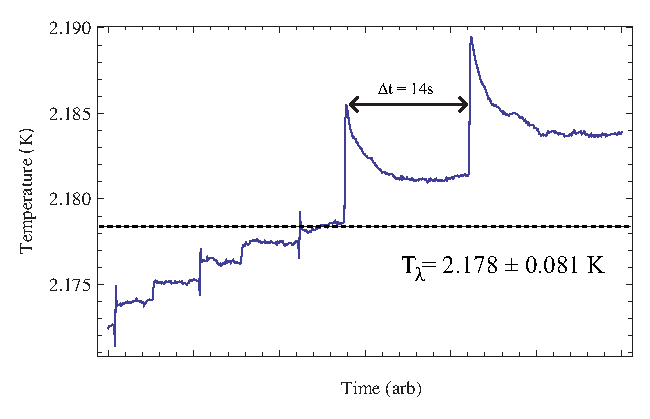
\includegraphics[height=70mm]{./figures/heatingdata.eps}
\caption{\small{Data from Figure~\ref{fig:rawdata}(b) after being converted from electric potential to temperature using the calibration in Section \ref{temperaturecalibration}.  From this data, $T_{\lambda}$ is determined to be $2.178\pm0.081$ K.}}
\label{fig:heatingdata}
\end{center}
\end{figure}

By analyzing data shown in Fig. \ref{fig:rawdata} (b) and using Eqn. \ref{eq:polyfit}, we can determine the value for $T_{\lambda}$ from $V_{\lambda}$, which is defined as the potential difference across the germanium resistor at which the helium in the cell transitions from helium II to helium I. 

As the temperature of He II increases to $T_{\lambda}$, the change in temperature $\Delta T$ decreases for a constant heat pulse $Q$.  This implies that the change in electric potential, $\Delta V$, decreases as it approaches $V_{\lambda}$.  The transition from He I to He II is denoted by a change in the heat pulse's signature.  As seen in Fig. \ref{fig:rawdata}, $\Delta V$ transitions from discrete steps to discrete exponentially decaying steps.  This signature is repeated after converting electric potential to temperature as shown in Fig. \ref{fig:heatingdata}.  The reason for this change in signature is due to the drastic divergence of the heat capacity of helium at $T_{\lambda}$.  For temperatures less than $T_{\lambda}$, the energy of the heat pulse sent to the cell is immediately absorbed uiformly in the He II due to the inability of superfluids to sustain temperature gradients.  This corresponds to the discrete steps we see in Fig. \ref{fig:rawdata} and Fig. \ref{fig:heatingdata}.  For temperatures greater than $T_{\lambda}$, the liquid helium, no longer in its superfluid state, can support temperature gradients.  As a result, the heat pulse is not immediately absorbed by the helium and the time constant describing the transfer of heat from the copper cell to the contained helium is much longer. This results in an exponential cooling curve as we see in Fig. \ref{fig:rawdata} and Fig. \ref{fig:heatingdata}.  

From this analysis, we can determine the range in which $T_{\lambda}$ occurs: \emph{i.e.}, between the temperatures which we know correspond to either He I or He II.  More precisely, we know that a heat pulse followed by discrete step in electric potential (or temperature) is the signature of He II, while an exponentially decaying signature corresponds to He I. Therefore the transition must lie in between these signatures.  Observing the measured electric potential data in Fig. \ref{fig:rawdata}, the interval for $V_{\lambda}$ must be as shown.  With Eqn. \ref{eq:polyfit}, we can convert this potential to temperature in order to determine $T_{\lambda}$.  Figure \ref{fig:heatingdata} shows the interval for $T_{\lambda}$, which we calculate to be $2.178\pm0.081$ K (see Appendix \ref{errorinspecificheatcalculation} for error analysis). 

To calculate heat capacity we use the converted temperature data in order to determine the cell's change in temperature, $\Delta T$, caused by a heat pulse with known energy $Q$, from some initial temperature $T$. To do this intensive calculation, we created a \emph{Mathematica} program which would iteratively measure $\Delta T$ over the entire temperature range observed ($>50000$ data points) and all the heat pulses ($>500$). By designating a threshold which varies over different temperature regions, the program identifies occurrences of sudden jumps in temperature corresponding to a heat pulse's signature. Having identified a pulse, the steady state mean temperatures before and after the pulse are recorded\footnote{The determination of the steady state temperature varied according to the temperature relative to $T_{\lambda}$.} and $\Delta T$ is computed.  Heat capacity is then calculated for each $\Delta T$ where $C=Q/\Delta T$.  This process produces data relating the heat capacity to temperature.  Using this algorithm, we are able to determine this relationship for both the evacuated and filled copper cell (Fig. \ref{fig:lambdanorm}).
\begin{figure}[htbp]
\begin{center}
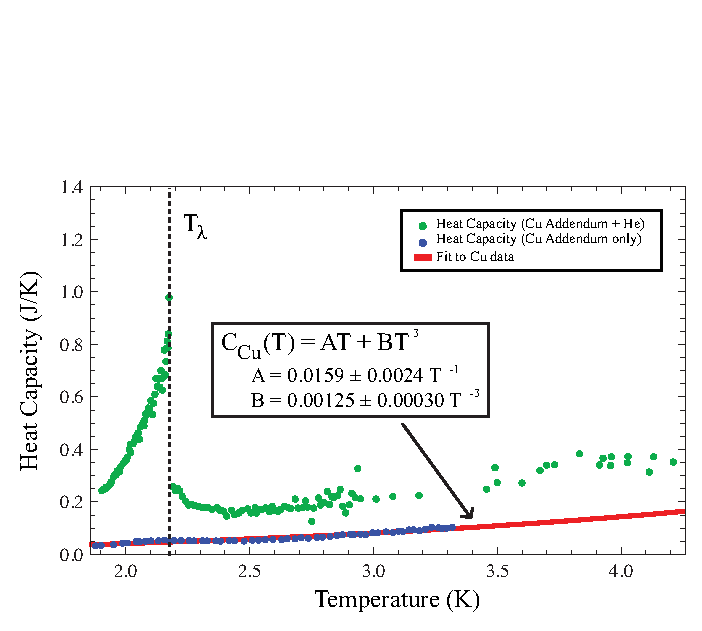
\includegraphics[height=80mm]{./figures/lambdanorm.eps}
\caption{\small{The heat capacity of the copper cell filled with He II and the heat capacity of the evacuated copper cell.  A polynomial with cubic and linear terms was fit to the copper data in order to ultimately remove the cell's contribution to the heat capacity data.}}
\label{fig:lambdanorm}
\end{center}
\end{figure}

To determine heat capacity of He without the copper cell we subtract heat capacity of the copper cell from that of the filled cell measurement.  To do this we fit a curve to the empty copper cell data.  At low temperatures, the heat capacity of copper is described by a combination of a linear and cubic temperature terms (see Section \ref{specificheatofmetals}).  Therefore we fit the copper heat capacity data to a $3^{rd}$-degree polynomial without  quadratic or constant terms using nonlinear regression.  We find that the heat capacity of the copper cell is given by
\begin{center}
\begin{equation}\label{eq:cufit}
C^{Cu}_{v} = 0.0159\pm0.0024 T+ 0.00125\pm0.00030 T^{3} 
\end{equation}
\end{center}

To remove the copper's contribution from the combined heat capacity at a specific temperature, we simply subtract the heat capacity of the cell, given by Eqn. \ref{eq:cufit}, for that temperature. Thus we are able to calculate the heat capacity of the He which is contained in the cell for the temperature region observed.  This heat capacity data must then be normalized to determine molar specific heat. As described in Section \ref{heatcapacityexperiment}, we use the ideal gas law to computer the number of moles of helium contained in the cell by measuring the pressure of a known volume of He at room temperature. That volume is then inserted into the cell through a capillary tubing.  We assume that almost all of the He is condensed in the cell due to the density of liquid helium being much greater than that of gaseous helium.  Knowing the number of moles of He in the cell, we can calculate its specific heat in J/mol K. This final data is shown in Fig. \ref{fig:lambdatrans}.
\begin{figure}[htbp]
\begin{center}
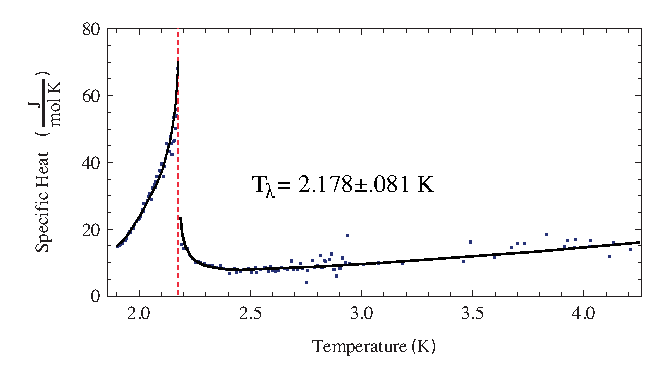
\includegraphics[height=80mm]{./figures/lambdatrans.eps}
\caption{\small{The specific heat of He II \emph{vs.} temperature. The transition from He I to He II occurs at $T_{\lambda} = 2.178 \pm 0.081$ K.  The values for specific heat each have a relative statistical error ranging from $10\%$  to $17\%$ based on the temperature of the helium (see Appendix \ref{errorinspecificheatcalculation} for error analysis). The measured points are overlaid onto the result from Atkins \cite{atkins}.}}
\label{fig:lambdatrans}
\end{center}
\end{figure}

\subsection{Superfluid and Normal Fluid Densities}\label{superfluiddensity}

We use the second sound speed and specific heat measurements derived
in Sections \ref{secondsoundanalysis} and \ref{heatcapacityanalysis}
to derive the fractions of superfluid and normal fluid as a function
of temperature. Given the speed of second sound, the specific heat,
and the entropy of helium II, it is possible to derive the ratio of
superfluid to normal fluid densities, $\rho_s/\rho_n$ by using the
relationship in Eqn. \ref{soundspeed}. From this ratio it is
straightforward to find the fractions $\rho_s/\rho$ and $\rho_n/\rho$
where $\rho$ is total density, since from \ref{eqn:density} we have
$\frac{\rho_n}{\rho} = 1 - \frac{\rho_s}{\rho}$.

As our experiment does not measure the entropy of helium II, we use the
results of Brooks and Donnelly \cite{brooks}. The entropy
values are cited at pressures of $0.0$ atm, $2.50$ atm, $5.0$ atm, and so on. Our
measurements were done at vapor pressures between $0.01$ atm and
$0.05$ atm, so the values for $0.0$ atm were used for the calculation.
In order to interpolate the entropy data, the logarithm of the
entropy, $\ln S$, was fitted to a second order polynomial:
\begin{equation}
\ln S = -0.8529T^2 + 6.092T - 8.82
\end{equation}

with an $r^2$-value of $0.9999$, which justifies the use of this fit
to interpolate entropy data.

In order to increase the precision of the specific heat data, between
$5$ and $10$ data points were averaged to give a value at each
temperature. The specific heat per gram and the second sound velocity
were combined with the entropy data to find the fraction of superfluid
and normal fluid (Fig. \ref{fig:density}). The errors from the
different sources were added in quadrature to give a maximum error of
$22\%$ on superfluid density. The curve can be seen to be in good
agreement with previously established results: most significantly the
shape, position of the $\lambda$-point, and temperature where $\rho_s
= \rho_n$ are in correspondence with previous literature \cite{andro}.
\begin{figure}[htbp]
\begin{center}
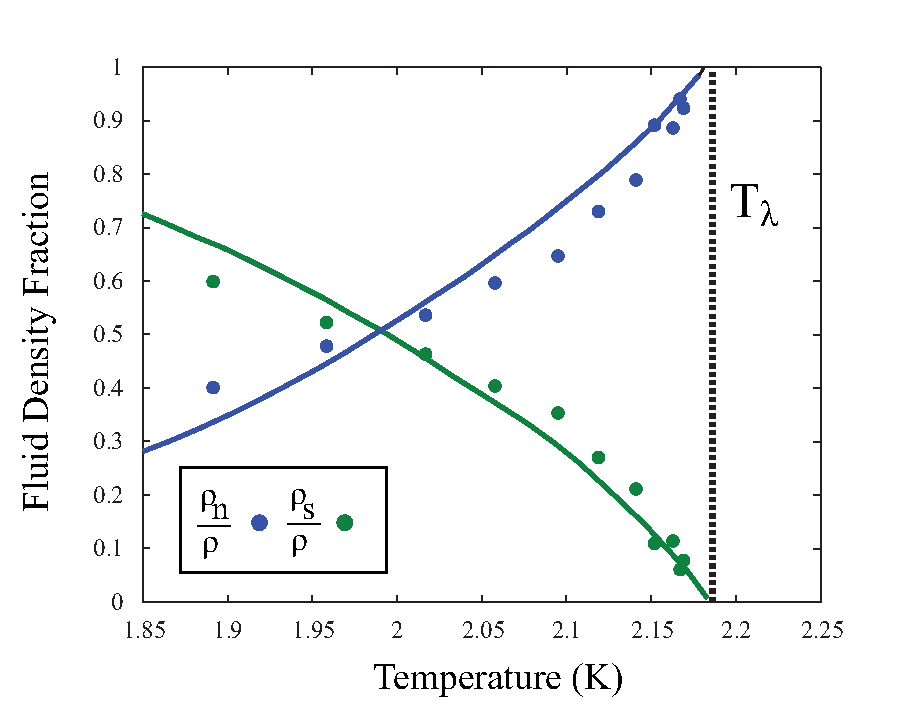
\includegraphics[height=90mm]{./figures/density.eps}
\caption{\small{Fraction of superfluid and normal fluid densities in
    helium II as a function of temperature, compared to
    Andronikoshvili's classic result from 1946 (solid
    line)\cite{andro}.}}
\label{fig:density}
\end{center}
\end{figure}
